%%
%% Automatically generated file from DocOnce source
%% (https://github.com/hplgit/doconce/)
%%
%%


%-------------------- begin preamble ----------------------

\documentclass[%
oneside,                 % oneside: electronic viewing, twoside: printing
final,                   % draft: marks overfull hboxes, figures with paths
10pt]{article}

\listfiles               %  print all files needed to compile this document
\usepackage{mathtools}
\usepackage{relsize,makeidx,color,setspace,amsmath,amsfonts,amssymb}
\usepackage[table]{xcolor}
\usepackage{bm,ltablex,microtype}
\usepackage{float}
\usepackage[pdftex]{graphicx}
\usepackage{epstopdf}

\usepackage{fancyvrb} % packages needed for verbatim environments

\usepackage[T1]{fontenc}
%\usepackage[latin1]{inputenc}
\usepackage{ucs}
\usepackage[utf8x]{inputenc}
\usepackage[english]{babel}
\usepackage{lmodern}         % Latin Modern fonts derived from Computer Modern

% Hyperlinks in PDF:
\definecolor{linkcolor}{rgb}{0,0,0.4}
\usepackage{hyperref}
\hypersetup{
    breaklinks=true,
    colorlinks=true,
    linkcolor=linkcolor,
    urlcolor=linkcolor,
    citecolor=black,
    filecolor=black,
    %filecolor=blue,
    pdfmenubar=true,
    pdftoolbar=true,
    bookmarksdepth=3   % Uncomment (and tweak) for PDF bookmarks with more levels than the TOC
    }
%\hyperbaseurl{}   % hyperlinks are relative to this root

\setcounter{tocdepth}{2}  % levels in table of contents



% prevent orhpans and widows
\clubpenalty = 10000
\widowpenalty = 10000

% --- end of standard preamble for documents ---


% insert custom LaTeX commands...

\raggedbottom
\makeindex
\usepackage[totoc]{idxlayout}   % for index in the toc
\usepackage[nottoc]{tocbibind}  % for references/bibliography in the toc

%-------------------- end preamble ----------------------

\begin{document}

% matching end for #ifdef PREAMBLE

\newcommand{\exercisesection}[1]{\subsection*{#1}}


% ------------------- main content ----------------------



% ----------------- title -------------------------

\thispagestyle{empty}

\begin{center}
{\LARGE\bf
\begin{spacing}{1.25}
PHYS 905 - Project 1
\end{spacing}
}
\end{center}

% ----------------- author(s) -------------------------

\begin{center}
{\bf Terri Poxon-Pearson}
\end{center}

    
% ----------------- end author(s) -------------------------

% --- begin date ---
\begin{center}
February 7, 2016
\end{center}
% --- end date ---

\vspace{1cm}

In this project we solved Poisson's equation via a tridiagonal matrix equation using three different algorithms:  A general tridiagonal solver, a more tailored version of this method, and LU Decomposition.  We explored the efficiency of these different methods and showed that we could reduce the necessary FLOPS to $4(n-1)$ where $n$ is the size of the matrix.  We also explored sources of error in this calculation and found that the a step size between $10^{-4}$ and $10^{-5}$ would minimize the error in our calculation.

\tableofcontents
 
\section{Introduction}
In this report we study different algorithms which can be used to solve linear, second order, differential equations.  As as example, we look at the example of Poisson's equation with Dirichlet boundary conditions.  For each method used, we cast Poisson's equation as a tridiagonal matrix equations.  First we employ a general algorithm for solving tridiagonal matrices.  Next, we specialize this algorithm to the specific features of this problem and study the effect on the number of Floating Point Operations per Second (FLOPS) which manifests in the CPU time.  Finally, we use a an algorithm for LU decomposition, a much more general method which does not require a tridiagonal form of the matrix.  We study how this powerful algorithm scales with matrix size.

In the following report, we introduce the matrix equation we solve, outine the general algorithm for solving tridiagonal matrices, and discuss how this algorithm can be tailored for our specific case.  These discussions will include discussions of the FLOPS required for each calculation.  We will end the Methods portion of this report with a brief introduction to the LU decomposition algorithm.  Then we wil discuss the implementation of these algorithms and the codes we used for our calculations.  We will then present our results which include a study of convergence to the analytical solutions, a comparison of computational speeds between different algorithms, and a detailed discussion of errors in the calculation.   Finally, we will present some conclusions and perspectives. 

\section{Methods}

\subsection{Poisson's Equation in Differential Form}

In this project we will be using Poisson's equation as an example of a linear, second order, differential equation.  This equation describes the electrostatic potential generated by a charge distribution and can be written as 

\begin{equation*}
\nabla^2 \Phi = -4\pi \rho (\mathbf{r}).
\end{equation*}

If we assume spherical symmetry this equation can be reduced to a one dimensional equation in r which can be generalized to 

\begin{equation*}
-u''(x) = f(x).
\end{equation*}

In this project we described Dirichlet boundary conditions, meaning that 

\begin{equation*}
-u''(x) = f(x), \hspace{0.5cm} x\in(0,1), \hspace{0.5cm} u(0) = u(1) = 0.
\end{equation*}

In our case, we will assume that sources term is $f(x) = 100e^{-10x}$, giving the closed form solution  $u(x) = 1-(1-e^{-10})x-e^{-10x}$.  We will use this exact solution to study the results of our algorithm.

\subsection{Poisson's Equation in Matrix Form}

In order to solve the differential equations, the functions must be discretized.  In this work, $u$ will be approximated byt $v_i$ where $x_i=ih$.  The discretized second derivative can be approximated using the three point formula

\begin{equation*}
\frac{d^2u}{dx^2} \approx \frac{v_{i+1} + v_{i-1} - 2v_i}{h^2} + O(h^2).
\end{equation*}
 
A full derivation of this expression can be found in \cite{LectureNotes}. Plugging this into our generalized Poisson's equation, we are left with

\begin{equation*}
   -\frac{v_{i+1}+v_{i-1}-2v_i}{h^2} = f_i  \hspace{0.5cm} \mathrm{for} \hspace{0.1cm} i=1,\dots, n.
\end{equation*}

This now gives us a set of equations corresponding to each $f_i$.  This set of equations can be cast as a matrix equation
\begin{equation*}
   \mathbf{A}\mathbf{v} = \tilde{\mathbf{b}}.
\end{equation*}
 Because there are only up to 3 $v_i$ terms in each equation corresponding to each $f_i$, this matrix equation will be tridiagonal and have the form

\[
    \mathbf{A} = \begin{bmatrix}
                           2& -1& 0 &\dots   & \dots &0 \\
                           -1 & 2 & -1 &0 &\dots &\dots \\
                           0&-1 &2 & -1 & 0 & \dots \\
                           & \dots   & \dots &\dots   &\dots & \dots \\
                           0&\dots   &  &-1 &2& -1 \\
                           0&\dots    &  & 0  &-1 & 2 \\
                      \end{bmatrix}
\]

and $\tilde{b}_i=h^2f_i$.

\subsection{General Tridiagonal Matrix Solver}

We can re-write the matrix expression in terms vectors $a,b,c$ of length $n$.  These vectors will not include the endpoints, as those values are already fixed by the boundary conditions. The equation becomes

\[
    \mathbf{A} = \begin{bmatrix}
                           d_1& e_1 & 0 &\dots   & \dots &\dots \\
                           e_1 & d_2 & e_2 &\dots &\dots &\dots \\
                           & e_2 & d_3 & e_3 & \dots & \dots \\
                           & \dots   & \dots &\dots   &\dots & \dots \\
                           &   &  &e_{n-2}  &d_{n-1}& e_{n-1} \\
                           &    &  &   &e_{n-1} & d_n \\
                      \end{bmatrix}\begin{bmatrix}
                           v_1\\
                           v_2\\
                           \dots \\
                          \dots  \\
                          \dots \\
                           v_n\\
                      \end{bmatrix}
  =\begin{bmatrix}
                           \tilde{b}_1\\
                           \tilde{b}_2\\
                           \dots \\
                           \dots \\
                          \dots \\
                           \tilde{b}_n\\
                      \end{bmatrix}.
\]

This equation can be solved using a simplified form of Gaussian elimination which involves two steps: a decomposition and forward substitution, followed by a backward substitution.  In the case of our matrix, we want to first eliminate the $e_1$ from the second row.  To do this, we multiply the first equation by $e_1/e_1$ and subtract it from the second equation.  This leaves us with

\[
    \mathbf{A} = \begin{bmatrix}
                           d_1& e_1 & 0 &\dots   & \dots &\dots \\
                           0 & d_2-\frac{e_1^2}{d_2} & e_2 &\dots &\dots &\dots \\
                           & e_2 & d_3 & e_3 & \dots & \dots \\
                           & \dots   & \dots &\dots   &\dots & \dots \\
                           &   &  &e_{n-2}  &d_{n-1}& e_{n-1} \\
                           &    &  &   &e_{n-1} & d_n \\
                      \end{bmatrix}\begin{bmatrix}
                           v_1\\
                           v_2\\
                           \dots \\
                          \dots  \\
                          \dots \\
                           v_n\\
                      \end{bmatrix}
  =\begin{bmatrix}
                           \tilde{b}_1\\
                           \tilde{b}_2-\tilde{b}_1\frac{e_1}{d_1}\\
                           \dots \\
                           \dots \\
                          \dots \\
                           \tilde{b}_n\\
                      \end{bmatrix}.
\]

These new diagonal elements are will be renamed $\tilde{d}_i$ and the new sorce terms will be renamed $\tilde{b^*}$.  This process is then repeated for each row of the matrix, finally leaving us with

\[
    \mathbf{A} = \begin{bmatrix}
                           d_1& e_1 & 0 &\dots   & \dots &\dots \\
                           0 & \tilde{d}_2 &\dots &\dots &\dots \\
                           & 0 & \tilde{d}_3 & e_3 & \dots & \dots \\
                           & \dots   & \dots &\dots   &\dots & \dots \\
                           &   &  & 0  &\tilde{d}_{n-1}& e_{n-1} \\
                           &    &  &   &0 & \tilde{d}_n \\
                      \end{bmatrix}\begin{bmatrix}
                           v_1\\
                           v_2\\
                           \dots \\
                          \dots  \\
                          \dots \\
                           v_n\\
                      \end{bmatrix}
  =\begin{bmatrix}
                           \tilde{b}_1\\
                           \tilde{b}^*\\
                           \dots \\
                           \dots \\
                          \dots \\
                           \tilde{b}^*_n\\
                      \end{bmatrix}.
\]

Where the general expressions for the matrix elements are:


\begin{equation} \label{eqn:General12}
\tilde{d}_i = d_i - \frac{e^2_{i-1}}{\tilde{d}_{i-1}}
\qquad \text{and} \qquad
\tilde{b}^*_i = \tilde{b}_i - \tilde{b}_{i-1}^* \frac{e_{i-1}}{\tilde{d}_{i-1}} 
\qquad \text{for} \qquad i=2,3,...n
\end{equation}



Next, we can do a backward substitution beginning with the final row of the matrix equation.  Solving the the unknown function, we get that $v_n=\tilde{b}^*_n/\tilde{d}_n$.  Now that $v_n$ is knows, we substitute this value into the equation from the second to last row and solve for $v_{n-1}$.  We can continue this backward substitution until all values $v_i$ are know.  The general formula for these elements are

\begin{equation}\label{eqn:General3}
v_i=\frac{\tilde{b}^*_i - e_i u_{i+1}}{\tilde{d}_i}  \qquad\text{for} \qquad i=n-2,n-1,...1.
\end{equation}

In the next section we will explore the efficiency of an algorithm which uses this method.

\subsection{FLOPS in General Algorithm}

The FLOPS for the algorithm are determined by the operations from the matrix decomposition, substitution, and backwards substitution.  This does not include the initialization of variables.  For the general algorithm there are three expressions which contribute to the floating point operations: The two equations in \ref{eqn:General12} and Equation \ref{eqn:General3}.  Each of these expressions have 3 operations which is repeated in each loop of the algorithm.  The first equations loop from $i=2-n$ and the third loops from $i=(n-1)-1$, for a total of n-1 loops for each.  This leaves us with $9(n-1)$ total floating point operations.

\subsection{Tailoring General Algorithm}

There are several steps that can be done to improve the algorithm's efficiency by taking advantage of the specific features of this matrix.  First, we know that all of diagonal elements will be 2 and all of the nonzero off diagonal elements will be -1.  Taking advantage of all $e_i=1$ lets us simplify the \ref{eqn:General12} and \ref{eqn:General3} to

\begin{equation} \label{eqn:Specific12}
\tilde{d}_i = d_i - \frac{1}{\tilde{d}_{i-1}}
\qquad \text{and} \qquad
\tilde{b}^*_i = \tilde{b}_i + \frac{ \tilde{b}_{i-1}^*}{\tilde{d}_{i-1}} 
\qquad \text{for} \qquad i=2,3,...n
\end{equation}

\begin{equation}\label{eqn:Specific3}
v_i=\frac{\tilde{b}^*_i + u_{i+1}}{\tilde{d}_i}  \qquad\text{for} \qquad i=n-2,n-1,...1.
\end{equation}

which leaves us with $6(n-1)$ operations.  Finally, we can precalculate $\tilde{d}_i$  with the observation that 

\begin{equation*}
\tilde{d}_i=\frac{i+1}{i}
\end{equation*}

Finally we are left with $4(n-1)$ floating point operations.

\subsection{LU Decomposition}

The third method we use for solving Poisson's equation is LU Decomposition.  This method is much more general than the past two and it is not necessary for the matrix to be tridiagonal. The process decomposes the initial matrix $\mathbf{A}$ into a product of and upper and lower triangular matrices $\mathbf{L} \cdot \mathbf{U}$.  Then if we want to solve the equation

\begin{equation*}
\begin{split}
&\mathbf{A} \cdot \mathbf{x} = \mathbf{y} \\
&\mathbf{L} \cdot \mathbf{U} \cdot \mathbf{x} = \mathbf{y}\\
& \mathbf{L} \cdot \mathbf{z} = \mathbf{y}
\end{split}
\end{equation*}

where $\mathbf{z}=\mathbf{U} \cdot \mathbf{x}$.  Then we can use a similar Gaussian elimination method to solve this, simpler, matrix equation.  This is a commonly used method and a full explanation of the procedure for decomposing and solving the matrix equation can be found in \cite{LectureNotes}.

Because this algorithm does not take advantage of the sparse nature of the tridiagonal matrix, it is much more computationally intensive and scales as $(2/3) n^3$.  The details of this scaling are given in \cite{Chiarandini}


\section{Code and Implementation}

All of the programs, results, and benchmarks for this work can be found in my GIT repository (https://github.com/poxonpea/PHYS905).  All codes for this project were written in FORTRAN.

\subsection{Implementing General Algorithm}

The code containing the main algorithm for solving the general tridiagonal matrix is shown here.

\begin{figure}[H]
  \centering
    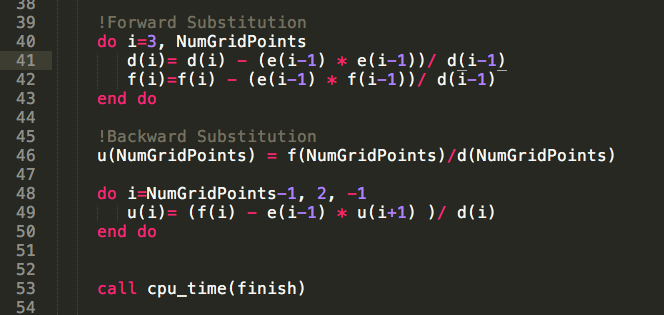
\includegraphics[width=1.2\textwidth]{GeneralAlgorithm}
\end{figure}

This does not include any of the initialization, but has the implementation of Equations \ref{eqn:General12} and Equation \ref{eqn:General3}.  This code also includes a function for producing the source term, calculating the exact solution and producing the relative error for the calculations.

\subsection{Implementing Tailored Algorithm}

The code containing the main algorithm for solving the tailored tridiagonal matrix is shown here.

\begin{figure}[H]
  \centering
    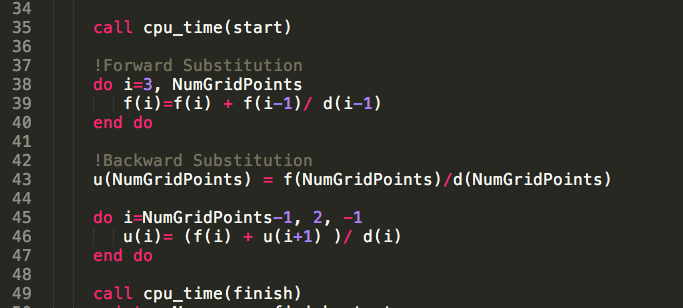
\includegraphics[width=1.2\textwidth]{SpecificAlgorithm}
\end{figure}

This code has almost the same structure as the general case, except for the section shown above and with different initializations.

\subsection{Implementing LU Decomposition}

For this calculation, I used the subroutines \texttt{lu\_decompose} and \texttt{lu\_linear\_equation} from the FORTRAN library provided for this course.  I just had to write a few lines which filled the tridiagonal matrix before feeding it into these subroutines.

\subsection{Calculating Relative Error}

The results from these algorithms can be compared to the analytic solution to understand the error in our calculations.  In this work, we study the log of the relative error which is defined by

\[
   \epsilon_i=log_{10}\left(\left|\frac{v_i-u_i}
                 {u_i}\right|\right),
\]

In the code, we calculated this value for each step size.  We can use this value to measure how well our calculation is reproducing the analytical solution and to keep track of our numerical precision.  This will be discussed in more detail in the following section.

\section{Results and Discussion}

\subsection{Convergence}

The Figure \ref{fig:comp} below shows the convergence of our different methods.  The analytic solution is plotted in black and solutions using different choices of step sizes are compared.  It is worth noting that this plot should be the same for each method because all of these algorithms approximate the differential equation as a tridiagonal matrix equation.  These methods converge quickly, with 10 grid points giving a rough description of the exact solution and 100 grid points being almost indistinguishable from the exact solution on this scale.

\begin{figure}[H]\label{fig:comp}
  \centering
    \includegraphics[width=1.2\textwidth]{comp.eps}
    \caption{Convergence for different choices of step sizes compared to the analytic solution.}
\end{figure}

Figure \ref{fig:compzoom} shows a zoomed in view of the results to we can distinguish between $n=100$ and $n=1000$ results.  In this view we can see that the $n=100$ result slightly under predicts the exact solution. 

\begin{figure}[H]\label{fig:compzoom}
  \centering
    \includegraphics[width=1.2\textwidth]{compzoom.eps}
    \caption{A zoomed in view of the convergence to the exact solution}
\end{figure}

\subsection{Computational Speeds}

Table \ref{table:test}, below, compares the speeds of the three different methods used in this study.  All times are reported in seconds. 

\begin{center} 
\begin{tabular}{ |c|c|c|c| }
\hline
Size of Matrix ($10^n$) & General & Tailored & LU \\
\hline
1& 3.00 E -6 & 3.00 E -6 & 2.40 E -5\\ 
2 & 4.00 E -6 & 4.00 E -6 & 1.71 E -3 \\ 
3 & 3.90 E -5 & 1.90 E -5 & 1.93\\ 
4 & 3.79 E -4 & 2.09 E -4 & N/A\\ 
5 & 3.38 E -3 & 1.51 E -3  & N/A\\ 
6 & 2.87 E -2 & 1.53 E -2 & N/A\\ 
7 & 3.16 E -1 & 1.73 E -1& N/A\\ 
\hline
\end{tabular}
\label{table:test}
\end{center}

When we created the tailored algorithm, we saw a reduction of $9(n-1)$ floating point operations in the general algorithm to just $4(n-1)$.  As expected, this corresponded to a significant decrease in the computation time.  The tailored algorithm takes roughly half the time as the general algorithm.  It is worth noting that this is not evident for small n.  That is because the run time is so short, it runs into the limit of the clock's granularity.

As we would expect, the computation time for the LU decomposition method is much longer, even for small n.  This is because this algorithm does not take into account the sparse nature of the tridiagonal matrix and tries to diagonalize the full matrix.  My computer was not able to calculate the $n=10^4$ matrix.

\subsection{Error Analysis}

Figure \ref{fig:error}, below, shows a log log plot of the relative error for different choices of step size, h.  It is worth noting that all of the methods used should demonstrate the same behavior in the error analysis because they all approximate the differential equation as a tridiagonal matrix equation.

\begin{figure}[H]
\label{fig:error}
  \centering
    \includegraphics[width=1.2\textwidth]{RelativeError.eps}
    \caption{Log-Log Plot of the relative error for different stepsizes}
\end{figure}

To quantify the expected error, we consider two sources.  The first is the approximation error($\epsilon_{ap}$) which comes from the truncation of the Taylor series expansion used to derive the three point formula.  The second is round off error ($\epsilon_{ro}$) which results from the way the computer stores and manipulates numbers.  For the three point formula, the expected approximation error is 

\begin{equation*}
\epsilon_{ap}\approx \frac{u_0^{(4)}}{12}h^2
\end{equation*}

and the expected round off error is

\begin{equation*}
\epsilon_{ro}\approx \frac{2 \epsilon_M}{h^2}.
\end{equation*}

For a full derivation of these error sources, see \cite{ClassNotes}.  For this report, all work was done using double precision variables, so $\epsilon_M$ is $10^{-15}$.  The total error is just the sum of these two terms.  If we take the derivative of that total with respect to step size, $h$, and set it equal to 0, we can solve for the step size that minimizes the error.  That would give us 

\begin{equation*}
h= \Bigg( \frac{24 \epsilon_M}{u_0^{(4)}} \Bigg)^{1/4}.
\end{equation*}

Depending on the choice of $x$, the expected step size which minimizes the error is between $10^{-4}$ and $10^{-5}$.  We see that is reflected exactly in our results.  The approximation error dominates at large h and goes as $h^2$, so we expect to see a slope of 2 on a log log plot in this region.  That is reproduced almost exactly in our calculation.  At small step size, the round off error begins to compete for the leading source of error and interferes with this pattern, eventually leading to error that increases with decreased step size.

\section{Conclusions}

In this project we studies three different methods for solving a tridiagonal matrix equation.  We have shown that it is important to consider the specific features of the problem before choosing a solving method.  Although LU decomposition is powerful in its generality, its scaling with matrix size ($(2/3)n^3$) is steep and cannot handle large matrices.  The general algorithm for solving the tridiagonal matrix is much faster and converges quickly.  Still, we found that with minimal modification, the computation time could be cut in half. 

Additionally, we explored the relative error as a function of step size.  We found that for large step size, the error is dominated by approximation error, but after a critical step size, round off error begins to compete as a source of error and continuing to decrease the step size will actually contribute to additional error.  This will be an important behavior to keep in mind for future projects.

\begin{thebibliography}{9}

\bibitem{LectureNotes} 
Hjorth-Jensen, Mortehn. 
Computational Physics, Lecture Notes Fall 2015. 
August 2015.

\bibitem{Chiarandini} 
Chiarandini, Marco. 
LU Factorization, Linear and Integer Programming. 
http://www.imada.sdu.dk/~marco/DM554/Slides/dm554-lu.pdf.

\bibitem{ClassNotes} 
Hjorth-Jensen, Mortehn. 
Introduction to Programming. 
Computational Physics.
https://compphysics.github.io/ComputationalPhysicsMSU/doc/pub/languages/pdf/languages-minted.pdf.

\end{thebibliography}




% ------------------- end of main content ---------------

\end{document}

